% -*- root: rapport.tex -*-
\documentclass[a4paper, 12pt]{article}
\usepackage{graphicx}
\DeclareGraphicsExtensions{.pdf,.png,.jpg}
\usepackage{xcolor}   %May be necessary if you want to color links
\usepackage{hyperref}
\usepackage{mathtools}
\usepackage{listings}
\usepackage{pgfplots}
\usepackage{pgfplotstable}
\usepackage{booktabs}
%\usepackage{inconsolata}


\hypersetup{
    colorlinks=true, %set true if you want colored links
    linktoc=all,     %set to all if you want both sections and subsections linked
    citecolor=black,
    filecolor=black,
    linkcolor=black,
    urlcolor=blue
}

\lstdefinestyle{customc}{
  belowcaptionskip=1\baselineskip,
  breaklines=true,
  frame=single,
  language=C,
  showstringspaces=false,
  basicstyle=\footnotesize\ttfamily,
  keywordstyle=\bfseries\color{green!40!black},
  commentstyle=\itshape\color{purple!40!black},
  identifierstyle=\color{blue},
  stringstyle=\color{orange},
  tabsize=4
}
\lstset{escapechar=@,style=customc}

\title{The Energy Efficiency of a Raspberry Pi Cluster used for Search}
\author{Eivind Siqveland Larsen and Knut Nygaard,\\
        Department of Computer Science,\\
        NTNU,
        Trondheim}

\begin{document}
\maketitle
\clearpage
\tableofcontents
\clearpage
\listoffigures
\clearpage

\begin{abstract}
In this project we have taken taken a look on how a cluster of Raspberry Pi computers perform when tasked with providing a search engine with regards to energy efficiency. We have built a cluster of eight nodes as well as the high powered USB hub required to run it. We have measured throughput and power consumption and compared performance and energy efficiency to that of a MacBook Pro running Core i5 and flash storage.

We have written the search engine as well as the programs needed to balance load and generate traffic. All code running on the Raspberry Pis is written in C for optimal performance.

Through our implementation and testing we have found that our relatively cheap system achieves comparable results with a newer MacBook Pro with regards to energy efficiency and performance at lower work loads. At peak load however, the small computers can not keep up in neither workload nor power efficiency. The Raspberry Pis showed a peak efficiency of 350 queries per Joule when overclocked, where as the i5 maxed out at about 710 queries per Joule for 1 core, and 842 for max load on 2 cores.
\end{abstract}


\clearpage
\section{Acknowledgments}
We would like to thank Svein Erik Bratsberg and \O ystein Torbj\o rnsen for help and the opportunity to do this project.

We would also like to thank Yngve Finnestad for his excellent advice and assistance regarding everything related to electrical engineering.

\section{Summary}
What problem are we trying to solve?

What did we do?

How did it turn out?



\clearpage
\section{Introduction}
\label{sec:introduction}

This section discusses the background for our project, what goals we have and the method we employed to reach our goals.

Section \ref{sec:related} briefly explores related work. 
In Section \ref{sec:hardware}, we introduce the properties of the hardware we will be using, and look at alternatives.
Section \ref{sec:software} explains the software we have built for this project as well as configuration of the nodes.
Section \ref{sec:build} shows how we built the hardware of the system we will be using as well as the structure for that holds our cluster.
Section \ref{sec:experiments} contains experiments we ran on the cluster as well as the corresponding the results and discussion.
Section \ref{sec:conclusion} contains our conclusion as well as further work that could be applied to the cluster.

\subsection{Background}
The demand for computing power is ever increasing. And even though performance has grown steadily, energy efficiency has not seen the same improvements. 
The performance has increased many fold over the last decades, but energy efficiency has not been able to follow. This means that the more powerful computers, while powerful, consume larger and larger amounts of energy. Especially in the realm of supercomputers, it has typically displayed the feature that performance scale sub-linearly, while power consumption at best scale linearly.
There has however been some signs in the last few years that this trend might be turning around\cite{green500}. 
Scogland et al.\cite{green500} reportedly find it likely that using less intelligent cores is a likely contributor to the increase seen in energy efficiency in small to large supercomputers in the later years.

On the other end, small single board system on chip computers are getting increasingly popular. They are tiny, low powered and cheap. But do they pack a punch? And can they be used for as traditional cluster computers?

We will look at how a set of these low energy devices compare up to an ordinary laptop computer if we take energy consumption, performance into account, and can they be used for cost efficiently scaling a system to different workloads?

In this report we explain how we built a low power hardware system, the software to stress test it, and discuss this system's performance and energy efficiency compared to a reference system. Our focus will be on delivering query results from a information retrieval system, stressing the two likely slowest parts of the PI\:
It's disk access and network.

\subsection{Goals}
In this project we have several questions we want to answer:
\begin{enumerate}
\item How does a cluster of Raspberry Pi nodes compare to a MacBook Pro running i5?
\item Can we scale our cluster efficiently?
\end{enumerate}

Throughout the project we will try to find answers for these questions.

\subsection{Method}
We will build a cluster of Raspberry PIs including a custom power supply. We will implement our own search system modifying code from the exercises of CS3245 Information Retrieval (National University of Singapore). To benchmark our system we will write a load generator to generate queries for our system to answer. We will also measure power consumption and compare these results with a MacBook Pro. 




\clearpage
\section{Related work}
\label{sec:related}
In this section we will explore related work on the area. For building we have specifically taken a look at a project by Joshua Kiepert and his work at building a Raspberry PI based Beowulf cluster.
After follows a look at the FAWN project and their take and findings on using ``Wimpy Nodes'' for cluster-based, high performance computing, and also defining their niche.
Lastly follows a argument for the base of our project and why low-powered, slower computers should be looked into.

\subsection{Raspberry PI Beowulf cluster}
A lot of the inspiration to create a Raspberry PI cluster came from reading a report on a Beowulf cluster project from Boise State University.\cite{RPI_BEOWULF} In this project the performance of 32 Raspberry PI nodes put up against a node running an 3.1GHz Intel Xeon E3-1225 quad-core processor and 8GB of RAM. Along with comparing performance under parallel computing, they also had a look on power consumption. It will be interesting to see if we achieve comparable results. 

\subsection{FAWN: A Fast Array of Wimpy Nodes}
FAWN\cite{fawn} is a project that aims to reduce the energy consumption of cost-effective clusters with data-intensive workloads. 
Andersen et al. propose a new cluster architecture that utilizes low-power embedded CPUs, small amounts of flash storage, balancing computation power and I/O capabilities to allow massively parallel data access.
They use this architecture to implement a replicated, highly available key-value store on a cluster made of such devices.

Their key-value store implementation is based on workloads typically seen by other highly available key-value stores, such as Amazons Dynamo and Facebooks memcached. These are geared towards high amounts of random accesses with small data objects, typically less than 1 KB. All this while requiring the highest levels of availability and durability.
Today these systems are typically run on large amounts of commodity hardware, including spinning hard drives, which are notoriously bad for random access patterns.

The hardware used is an embedded device based on a SoC from PCEngine. It features a 500MHz AMD Geode LX processor, coupled with 256 MB RAM running at 400 MHz. The storage is done by a Compact Flash controller. Power consumption is quoted between 3W and 6W (peak load).

Through their work, \cite{fawn} shows they were able to provide roughly 350 queries per Joule which is 2 orders of magnitude more than traditional disk-based systems at the time of writing (2009). 

\subsection{Motivation}
Motivational factors for our project is interest in energy efficient scaling of systems.

The reason for small embedded computers with small amounts of flash storage is related to several problems within current computing.

The CPU performance compared to I/O gap is still increasing. CPUs continue to increase performance at a vastly higher rate than IO devices, such as storage and network equipment.
When these factors are bottlenecking the system, i.e. when the system is doing a lot of data intensive work, it often results in low CPU utilization.

With embedded devices using flash storage as persistent storage, this performance gap is a lot closer.
Together with the simpler and slower processors it results in fewer cycles spent waiting for IO to happen.

This also benefits the embedded computers in another way. Modern powerful CPUs have despite the improved efficiency of later years, still a fairly high base power consumption.
By base power consumption we mean that a CPU being utilized at 25\% consumes more than 50\% of the power consumed at 100\% utilization. 
This motivates keeping the CPU at high loads for energy efficiency means, but this can not happen if it being stuck waiting for IO.
Ergo, to ensure energy efficiency, one should keep the CPU as busy as possible.

\cite{fawn} also argues the simpler architecture of embedded CPUs is leaving a larger portion of the transistors to actually execute operations.
In more advanced CPUs a lot of die space and transistors is spent on cache storage, cache coherency protocols, and speculative execution, like out-of-order instructions and branch prediction.
All of this logic requires large amounts of energy to power, and is mostly there to help bridge the gap between CPU and disc/IO devices. But this does not help directly with operations in the CPU, and increases power consumption by a good amount.
The simpler CPUs, providing a larger proportion of transistors to executing operations, are thus more energy efficient while executing these because they have less overhead in powering additional transistors, i.e. they provide more instructions executed per Joule.






\section{Hardware}
\subsection{Raspberry PI}
\subsection{Alternative hardware}
\subsection{Cluster}
\subsection{Power}


\clearpage
\section{Software}
\label{sec:software}
For this project, we needed quite a bit a software to be sure we could generate somewhat realistic workloads.
We also thought it important with predictability and put a lot of effort towards having a controlled environment. This goes for both the software and hardware involved.

Having done a bit of performance analysis before, we are aware of how difficult it can be to get meaningful and consistent results when analyzing programs and hardware interactions. We therefore decided to base ourselves on using some code we had written earlier in a information retrieval course. It is a simple search engine and indexer written in python, that does full text searches on a indexed corpus.

\subsection{Alternatives}
There are a few open source projects already that are focused on information retrieval. We will here discuss some of the software we were considering using for this project.

\subsubsection{Lucene/Solr}
The most obvious software alternative might be the information retrieval system Lucene. Lucene is a heavier search engine written in Java, so it also requires a JVM to be running. The limited amount of less than 500MB of RAM was our main concern when we were discussing whether to use Lucene.

Additionally it is not a project and codebase we are familiar with.
This fact alone would make it hard for us to modify Lucene to our needs and be sure we got it right, and keep the level of control we wish for.

To make Lucene deployable in a distributed environment, a sideproject called Solr was started, and later included in the official Lucene project. 
It offers a way to easily deploy Lucene and it's capabilities in a distributed manner, using among other things ZooKeeper for coordinating the cluster.

The concerns mentioned above and our unfamiliarity with the projects Lucene and Solr made us decide against using them.

\subsubsection{Sphinx}
Another open source project is the Sphinx search engine\cite{sphinx}. Sphinx provides full-text searching with a number of interfaces, including a SQL storage engine that can deliver results through a MariaDB server and connection. Spinx also has a query language much like SQL.

But this library also seems like overkill for our intents and purposes, so we decided against this.

\subsection{Setup}
As the authors had most experience with Arch Linux and it's environment, we decided to go with the distribution provided by the Arch Linux for ARM project.
The OS is distributed as a ISO image, which is written to the SD card using the UNIX disk utility {\tt dd}:
\begin{lstlisting}
dd if=inputimage.iso of=/dev/outdisk bs=1M
\end{lstlisting}

\subsection{Doing a search}
Since a significant part of our project is related to searching, we find it reasonable to include a section on how a search engine works in general.

Our engine consist of two parts: indexing and searching.
The search engine executes and scores a set of documents for given queries. For this work, it uses the dictionary, and a postings file.
The other part is the indexer, which builds an inverted index, the dictionary, and the postings file\cite{IntroIR} over a collection of documents (corpus).

When performing the indexing task, a loop runs over every document in the corpus.
For every word encountered in a document, the indexer emits a term, which is made into a token.
A token what is left after post-processing a term. This processing usually includes stemming and removal of special characters.
The token is added to a dictionary and the document id is appended to the token's postings list. A counter is also kept along with the id to keep track of multiple occurrences of the same token in the same document.
The result of this loop is a dictionary of all unique tokens encountered, along with a postings list, naming all the documents that contain each token.

The dictionary contains the token, how many times it occurs in the collection, and a pointer to where this term is stored in the postings file.
The entries can be viewed as a tuple of the format:
$$<token, count, pointer>$$
The postings pointer is in our case an integer. This integer is the byte offset in the posting file where this terms posting list starts.

The postings entries are a list of tuples, in the format $$<docID, count>$$, giving the document id where the token occurred and the number of times it was seen in that document.

\begin{figure}[h]
    \center
    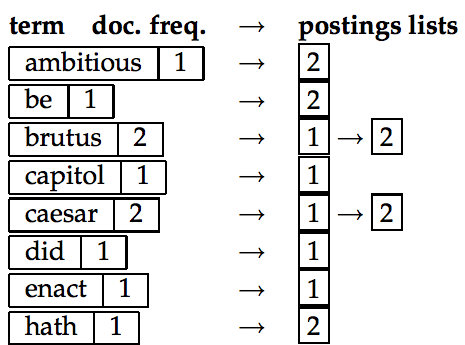
\includegraphics[width=0.5\textwidth]{software/index_postings_lists}
    \caption{A sample index and postings list. Figure taken from Introduction to IR\cite{IntroIR}.}
    \label{fig:index_postings_lists_sw}
\end{figure}

\subsection{Document scoring}
In the searching step one is usually working with a query containing one or more terms. For each token the corresponding postings list is fetched from disk (and cached). Each document is then scored according to a scoring scheme and a list of the documents sorted by the score is returned to the application.

To provide a rudimentary form of scoring, we have implemented the TF-IDF scoring system for queries. We are using the weighting scheme suggested by Introduction to Information Retrieval\cite{IntroIR}, {\tt lnc.ltc} in SMART notation\cite{tfidfsmart}.


\subsection{Operating system and environment}
Our operating system of choice is the Arch Linux for ARM project\cite{archarm}. This distribution provides us with a rolling release scheme, and eases development through the big and developer friendly package system AUR. If something is missing, it can be a lot easier to add it to all of the systems through the package manager.

The systems were mostly running on Linux kernel 3.6.11-18-ARCH, compiled for armv6l. This is as reported by running {\tt uname -a} on the target platform.

The systems also had the raspberrypi-firmware-tools packages, dated 20131021-1. Compilation was done with gcc:
\begin{lstlisting}[captionpos=b,caption={Output of {\tt gcc -v} and {\tt python --version}}]
$ gcc -v
Using built-in specs.
COLLECT_GCC=gcc
COLLECT_LTO_WRAPPER=/usr/lib/gcc/armv6l-unknown-linux-gnueabihf/4.7.2/lto-wrapper
Target: armv6l-unknown-linux-gnueabihf
Configured with: /build/src/gcc-4.7.2/configure --prefix=/usr --libdir=/usr/lib --libexecdir=/usr/lib --mandir=/usr/share/man --infodir=/usr/share/info --with-bugurl=https://bugs.archlinux.org/ --enable-languages=c,c++,fortran,lto,objc,obj-c++ --enable-shared --enable-threads=posix --with-system-zlib --enable-__cxa_atexit --disable-libunwind-exceptions --enable-clocale=gnu --disable-libstdcxx-pch --enable-libstdcxx-time --enable-gnu-unique-object --enable-linker-build-id --with-ppl --enable-cloog-backend=isl --disable-ppl-version-check --disable-cloog-version-check --enable-lto --enable-gold --enable-ld=default --enable-plugin --with-plugin-ld=ld.gold --with-linker-hash-style=gnu --disable-multilib --disable-libssp --disable-build-with-cxx --disable-build-poststage1-with-cxx --enable-checking=release --host=armv6l-unknown-linux-gnueabihf --build=armv6l-unknown-linux-gnueabihf --with-arch=armv6 --with-float=hard --with-fpu=vfp
Thread model: posix
gcc version 4.7.2 (GCC)

$ python --version
Python 2.7.5
\end{lstlisting}

\subsection{Booting and deployment}
To collaborate and distribute our code, we use a git repository stored at GitHub\cite{github}. We also agreed upon a set folder structure to make it easier to maintain and deploy our code, storing the git directory under {\tt /home/<user>/src/project}.
The username is the same for all nodes.

We created a systemd script that runs at boot, which does a repository pull and builds all the code, then run it. So to deploy a new update, we would cut the power to the rig and start it again.
This proved very efficient in practice and saved us a lot of work manually, or by scripts, logging in and updating and relaunching each system. The boot script is given in listing \ref{lst:bootscript}.
\begin{lstlisting}[captionpos=b,caption={Our Systemd boot script. It launches a script that makes sure datetime is set before launching the update script.},label={lst:bootscript}]
#-/etc/systemd/system/pinode.service
[Unit]
Description=PI search service
ConditionPathExists=/etc/rc.local

[Service]
Type=forking
ExecStart=/etc/rc.local
TimeoutSec=0
StandardOutput=tty
RemainAfterExit=yes
SysVStartPriority=99

[Install]
WantedBy=multi-user.target

#-/etc/rc.local
su king -c "/home/king/src/project/boot_pinode.py"

#-boot_pinode.py
projectdir = "/home/king/src/project"
hostname = socket.gethostname()

os.chdir(projectdir)

def update_git():
    subprocess.call(["git", "pull"])
    subprocess.call(["make"])

def launch_load_distr():
    subprocess.call(["bin/load_distributor_bin"])

def launch_search_engine():
    subprocess.call(["bin/search_bin"])

while True:
    update_git()

    if hostname[len(hostname)-1] == '0':
        launch_load_distr()
    else:
        launch_search_engine()

\end{lstlisting}

\subsection{Load generator}
The purpose of the load generator is to generate pseudo-random queries and send these to the load distributor to simulate load on the cluster. These queries are of varying length and contains tokens found in the dictionary.

The load generator runs on several threads, where one thread is responsible for receiving answers for the queries, and one or more threads are responsible for generating load for the system. The load generator is implemented in python and meant to be run on a node outside the cluster.

The load generator includes some configurable parameters, most importantly the frequency of the queries being sent and the number of threads sending queries simultaneously.

The load generator was later edited to also be able to send queries directly to the workers and then bypass the load distribution all together. This simulates moving the load distribution out to the client application. In this case, we have one thread for each worker that sends messages at a given interval.

\subsection{Load distribution}
One of the nodes in the cluster will be in charge of load distribution. The load distributor node will receive all the queries and then forward them to the worker nodes.
The node employs the very simple load balancing scheme of $$rand() \bmod N,$$ where N is the number of nodes in the cluster.
The messages from the load distributor to the worker nodes includes information of where to deliver the search results when they are ready.
This scheme is simple, but could also prove to be a bottleneck of the system. Seeing as all communication has to go through this node we could end up with the performance of the cluster being limited by the load distributor.

\subsection{Original search engine - python version}
The python version we were basing the program on relied heavily upon the python library Natural Language Toolkit\cite{nltk} (NLTK).
NLTK provides a lot of useful methods for processing natural languages in Python, including different tools for stemming and other tokenization tricks.
Stemming is the process of reducing inflected or conjugated words into their basic or root form. Examples include removal of prefixes, suffixes, tense and vowel changes. I.e. words like ``fishing'', ``fisher'' and ``fished'' all end up mapping to the same stem ``fish''.

The toolkit also provides stop word lists (words like and, or, on, i and so on) and improved splicing of natural language sentences. As this is a lot of work to implement, we have chosen to do indexing in python and deliver and calculate search results based only on the stemmed forms for the C program.

\subsection{Optimized C-port}
In practice we experienced serious performance issues with our python code, often showing response times in the hundreds of milliseconds. We therefore decided to rewrite the program using C. This proved it both challenging and useful to control what exactly is present in memory at every moment, in addition to the extra work of having to control memory allocation.

The program reads the dictionary structure into memory on startup. It provides O(1) lookup on query terms in a hash map, using the library {\tt uthash}\cite{uthash}.

\begin{lstlisting}[style=customc,captionpos=b,caption={Structure of a dictionary entry (term)},numbers=left]
typedef struct {
    char* term;
    uint32_t byte_offset;
    uint32_t occurences;
    postings_entry* posting;
    UT_hash_handle hhd;         /* makes this structure hashable */
} dictionary_entry;
\end{lstlisting}
\subsubsection{uthash}
{\tt uthash} is a small library with a set of convenient preprocessor macros for creating and managing hash tables in C.
{\tt uthash} does constant time $$O(1)$$ lookups, inserts and deletes, and comes with a number of different hash functions in case your key domain is not well suited for the default hash function.
{\tt uthash} can hash strings, integers, pointers and the bytes in a structure a pointer points to.

\subsubsection{Experiences}
The first testings of the C-port showed significant improvements in delivery speed.
It further confirmed that managing memory yourself is desirable for performance, and is especially important in an environment where resources are scarce.
When blasting the searching code with queries, we quickly maxed out the available memory.
These memory leaks were later fixed, and the program now experiences constant memory usage.

The difference in developing platform, with x86\_64 Darwin compared to the ARMv6 runtime environment did not impose any extra difficulties, except for a single case of some odd pointer behavior.
The rest of the time, the code behaved as expected from one platform to the other, for both Python and C.

For comparison between the two languages, we created a test set of 100,000 queries. We then ran this test set against the reference MacBook computer, and on the pi, both for Python and {C}.
The results are given in Table \ref{tbl:runtimes_ports}.

For the relatively quick {Core i5}, the python code need 10 times longer to run the queries than the C code, and seem reasonable compared to known sources.
The Python code is however detrimental to the performance for the weaker PI. The same 100,000 queries takes 84 seconds to run in C, but takes 24 times longer in python.

\begin{table}[h]
	\begin{center}
	\begin{tabular}{|r|r|r|r|}
	\hline
	   & \multicolumn{1}{|c|}{MacBook} & \multicolumn{1}{|c|}{PI (OC)}  & \multicolumn{1}{|c|}{PI} \\
	\hline
	C      & 4.782 & 55.932 & 84.748     \\
	\hline
	Python & 49.411 & 1268.892 & 2046.768   \\
	\hline
	\end{tabular}
	\caption{Runtime (in seconds) for C and Python code on 100,000 queries.}
	\label{tbl:runtimes_ports}
	\end{center}
\end{table}


\clearpage
\section{The build}
\subsection{Power supply}
After consulting a fellow student from the Electrical Engineering faculty, we acuired a power adapter able to provide enough amperes(hopefully) to run the entire cluster. After ordering some USB heads from Ebay we set out to create our own high powered USB hub. 

The Lacie power adapter comes with a 4 pin connector providing 12V and 5V. Since only the 5V is needed, we cut the cable and put on a new connector jack connecting only the 5V and ground. This also provided us with an easy way to remove the cable for when we need to turn off or move the cluster. 

Once we had a power source we set up a simple circut with only one USB head to test. After measuring and makeing sure everything was in order a Raspberry PI was connected. It booted and everything was working, so our proof of concept was done.  

Next came building the USB hub. 8 USB connectors were soldered to a [koblingskort] along with the female part of the connector jack providing the power. Everything was connected in paralell using the twisted pair cables salvaged from an ethernet cable.  

\begin{figure}[h]
	\centering
    \includegraphics[width=0.5\textwidth]{thebuild/result.png}
    \caption{Power supply: end result}
    \label{fig:build_power_supply}
\end{figure}

\subsection{The cluster}

\begin{figure}[h]
	\centering
    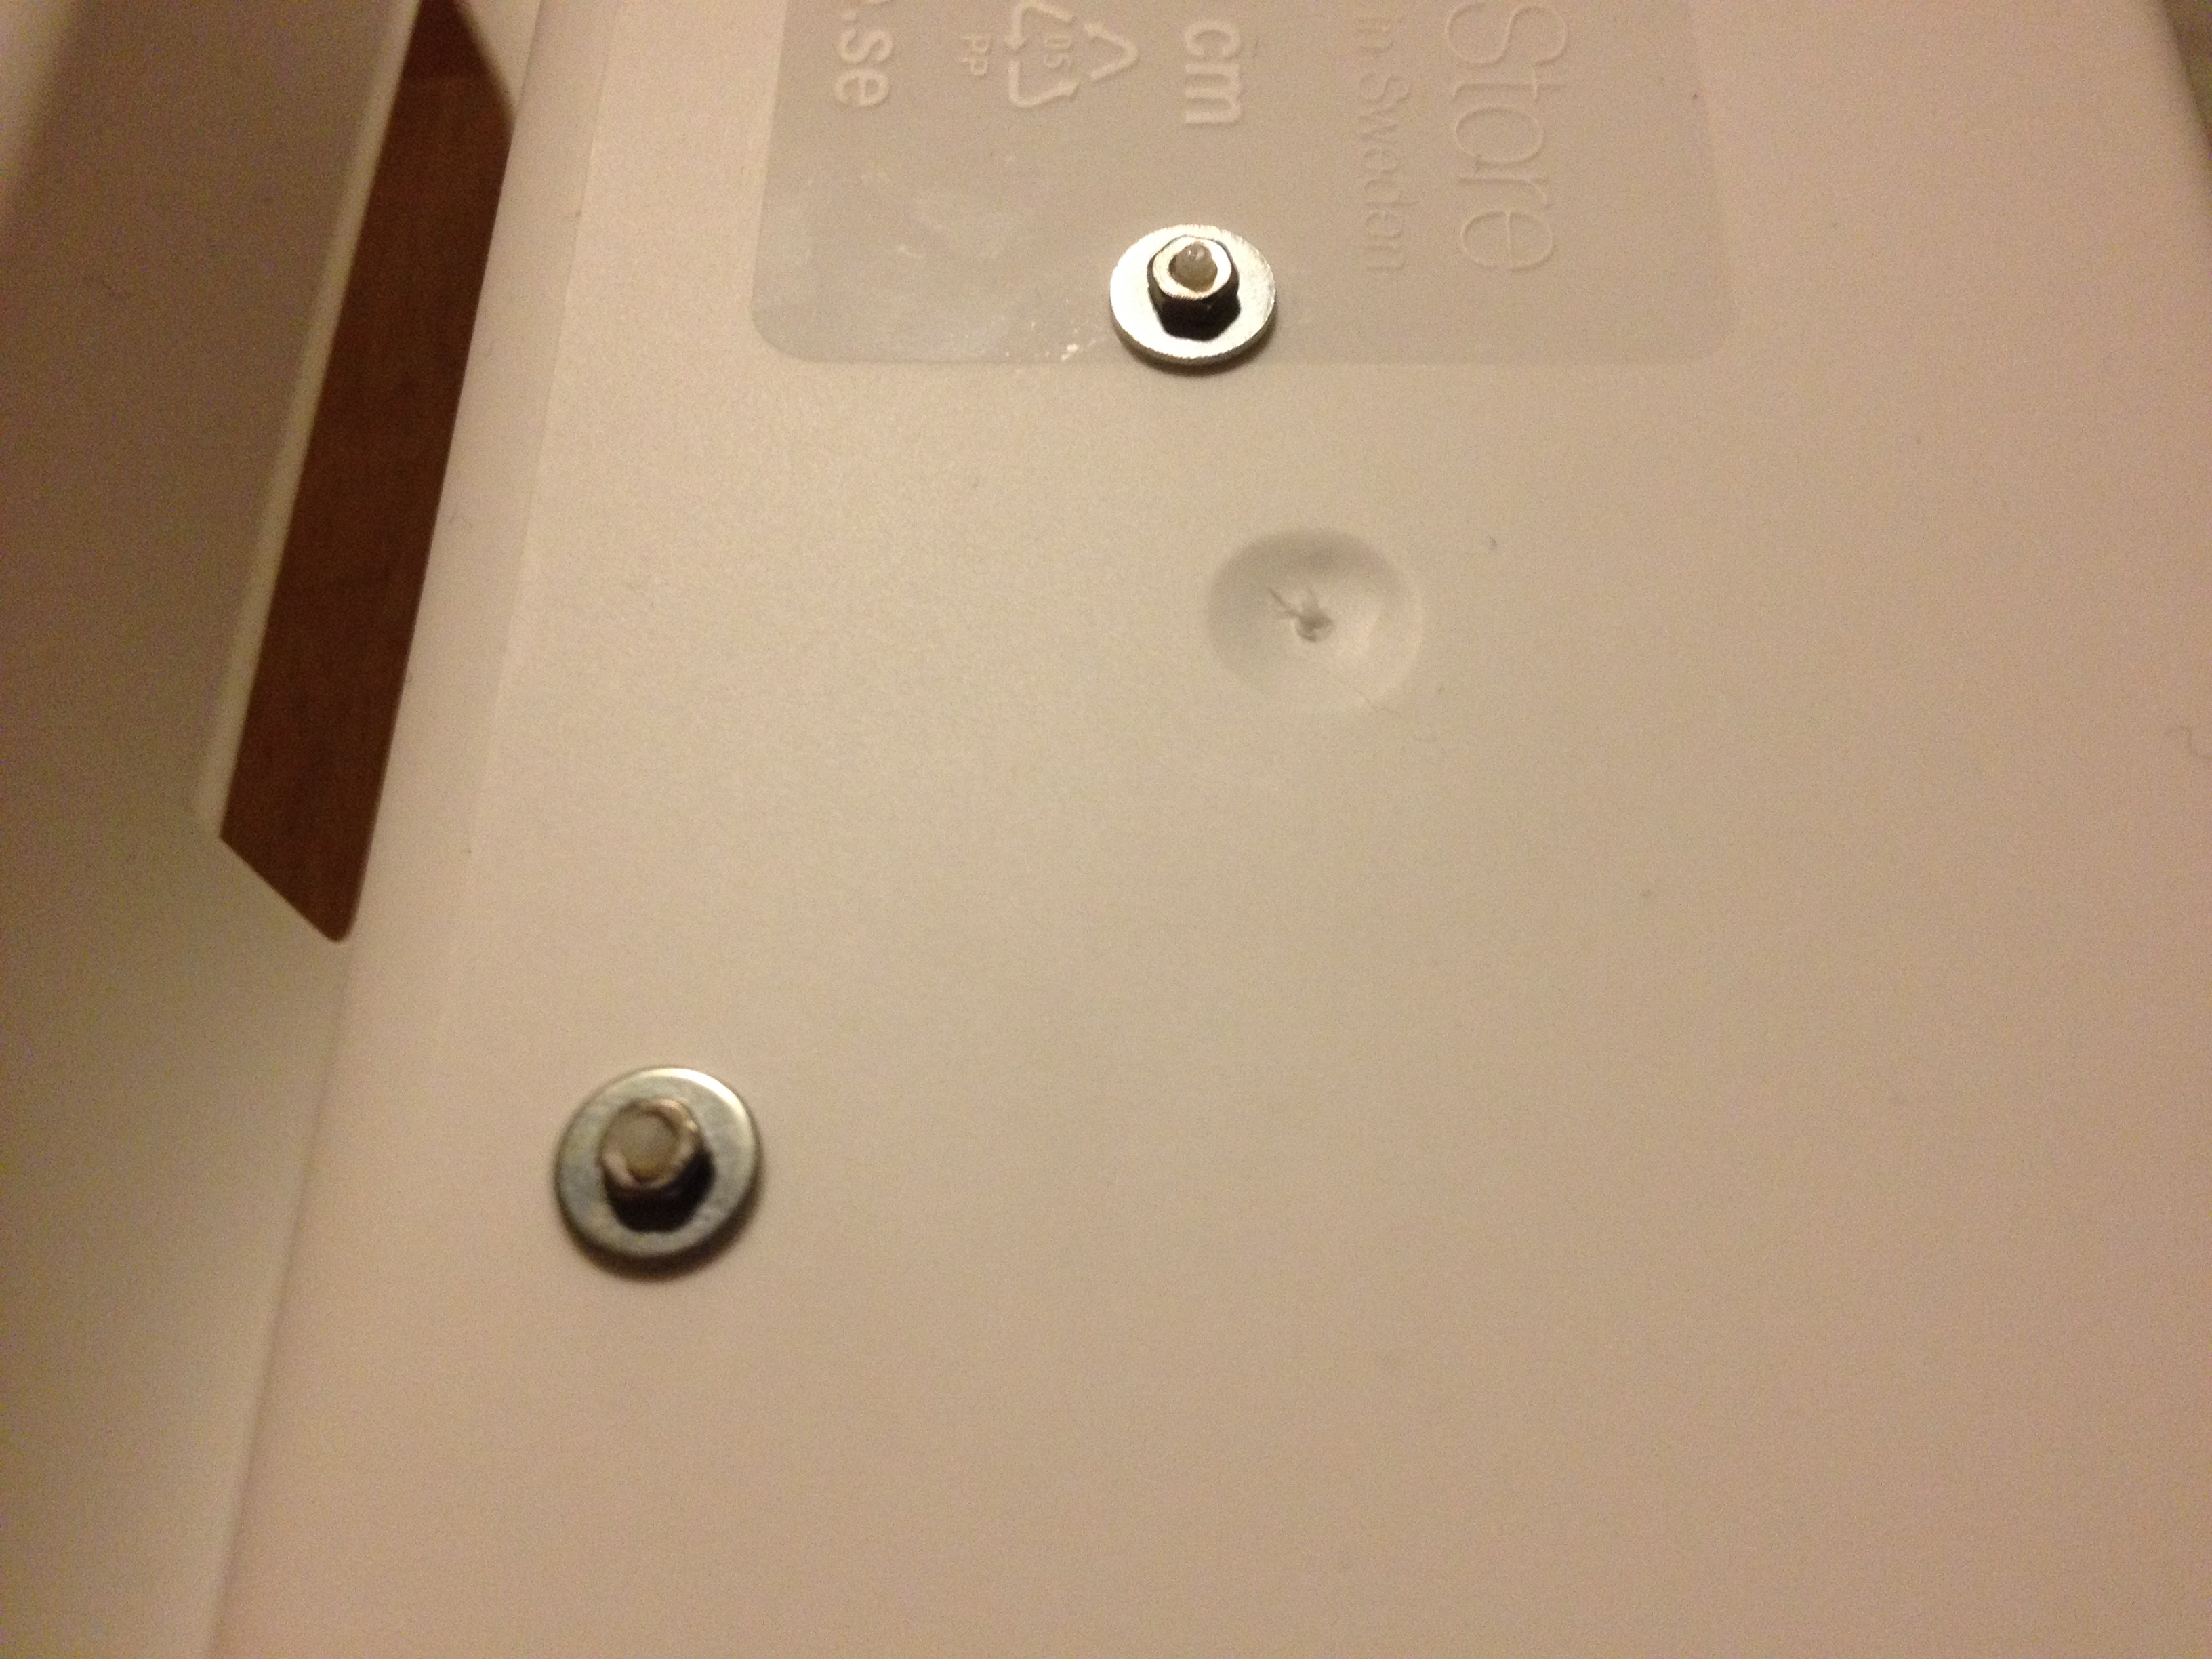
\includegraphics[width=0.5\textwidth]{thebuild/cluster_under.jpg}
    \caption{Under the clusterbox}
    \label{fig:build_cluster_under}
\end{figure}

\begin{figure}[h]
	\centering
    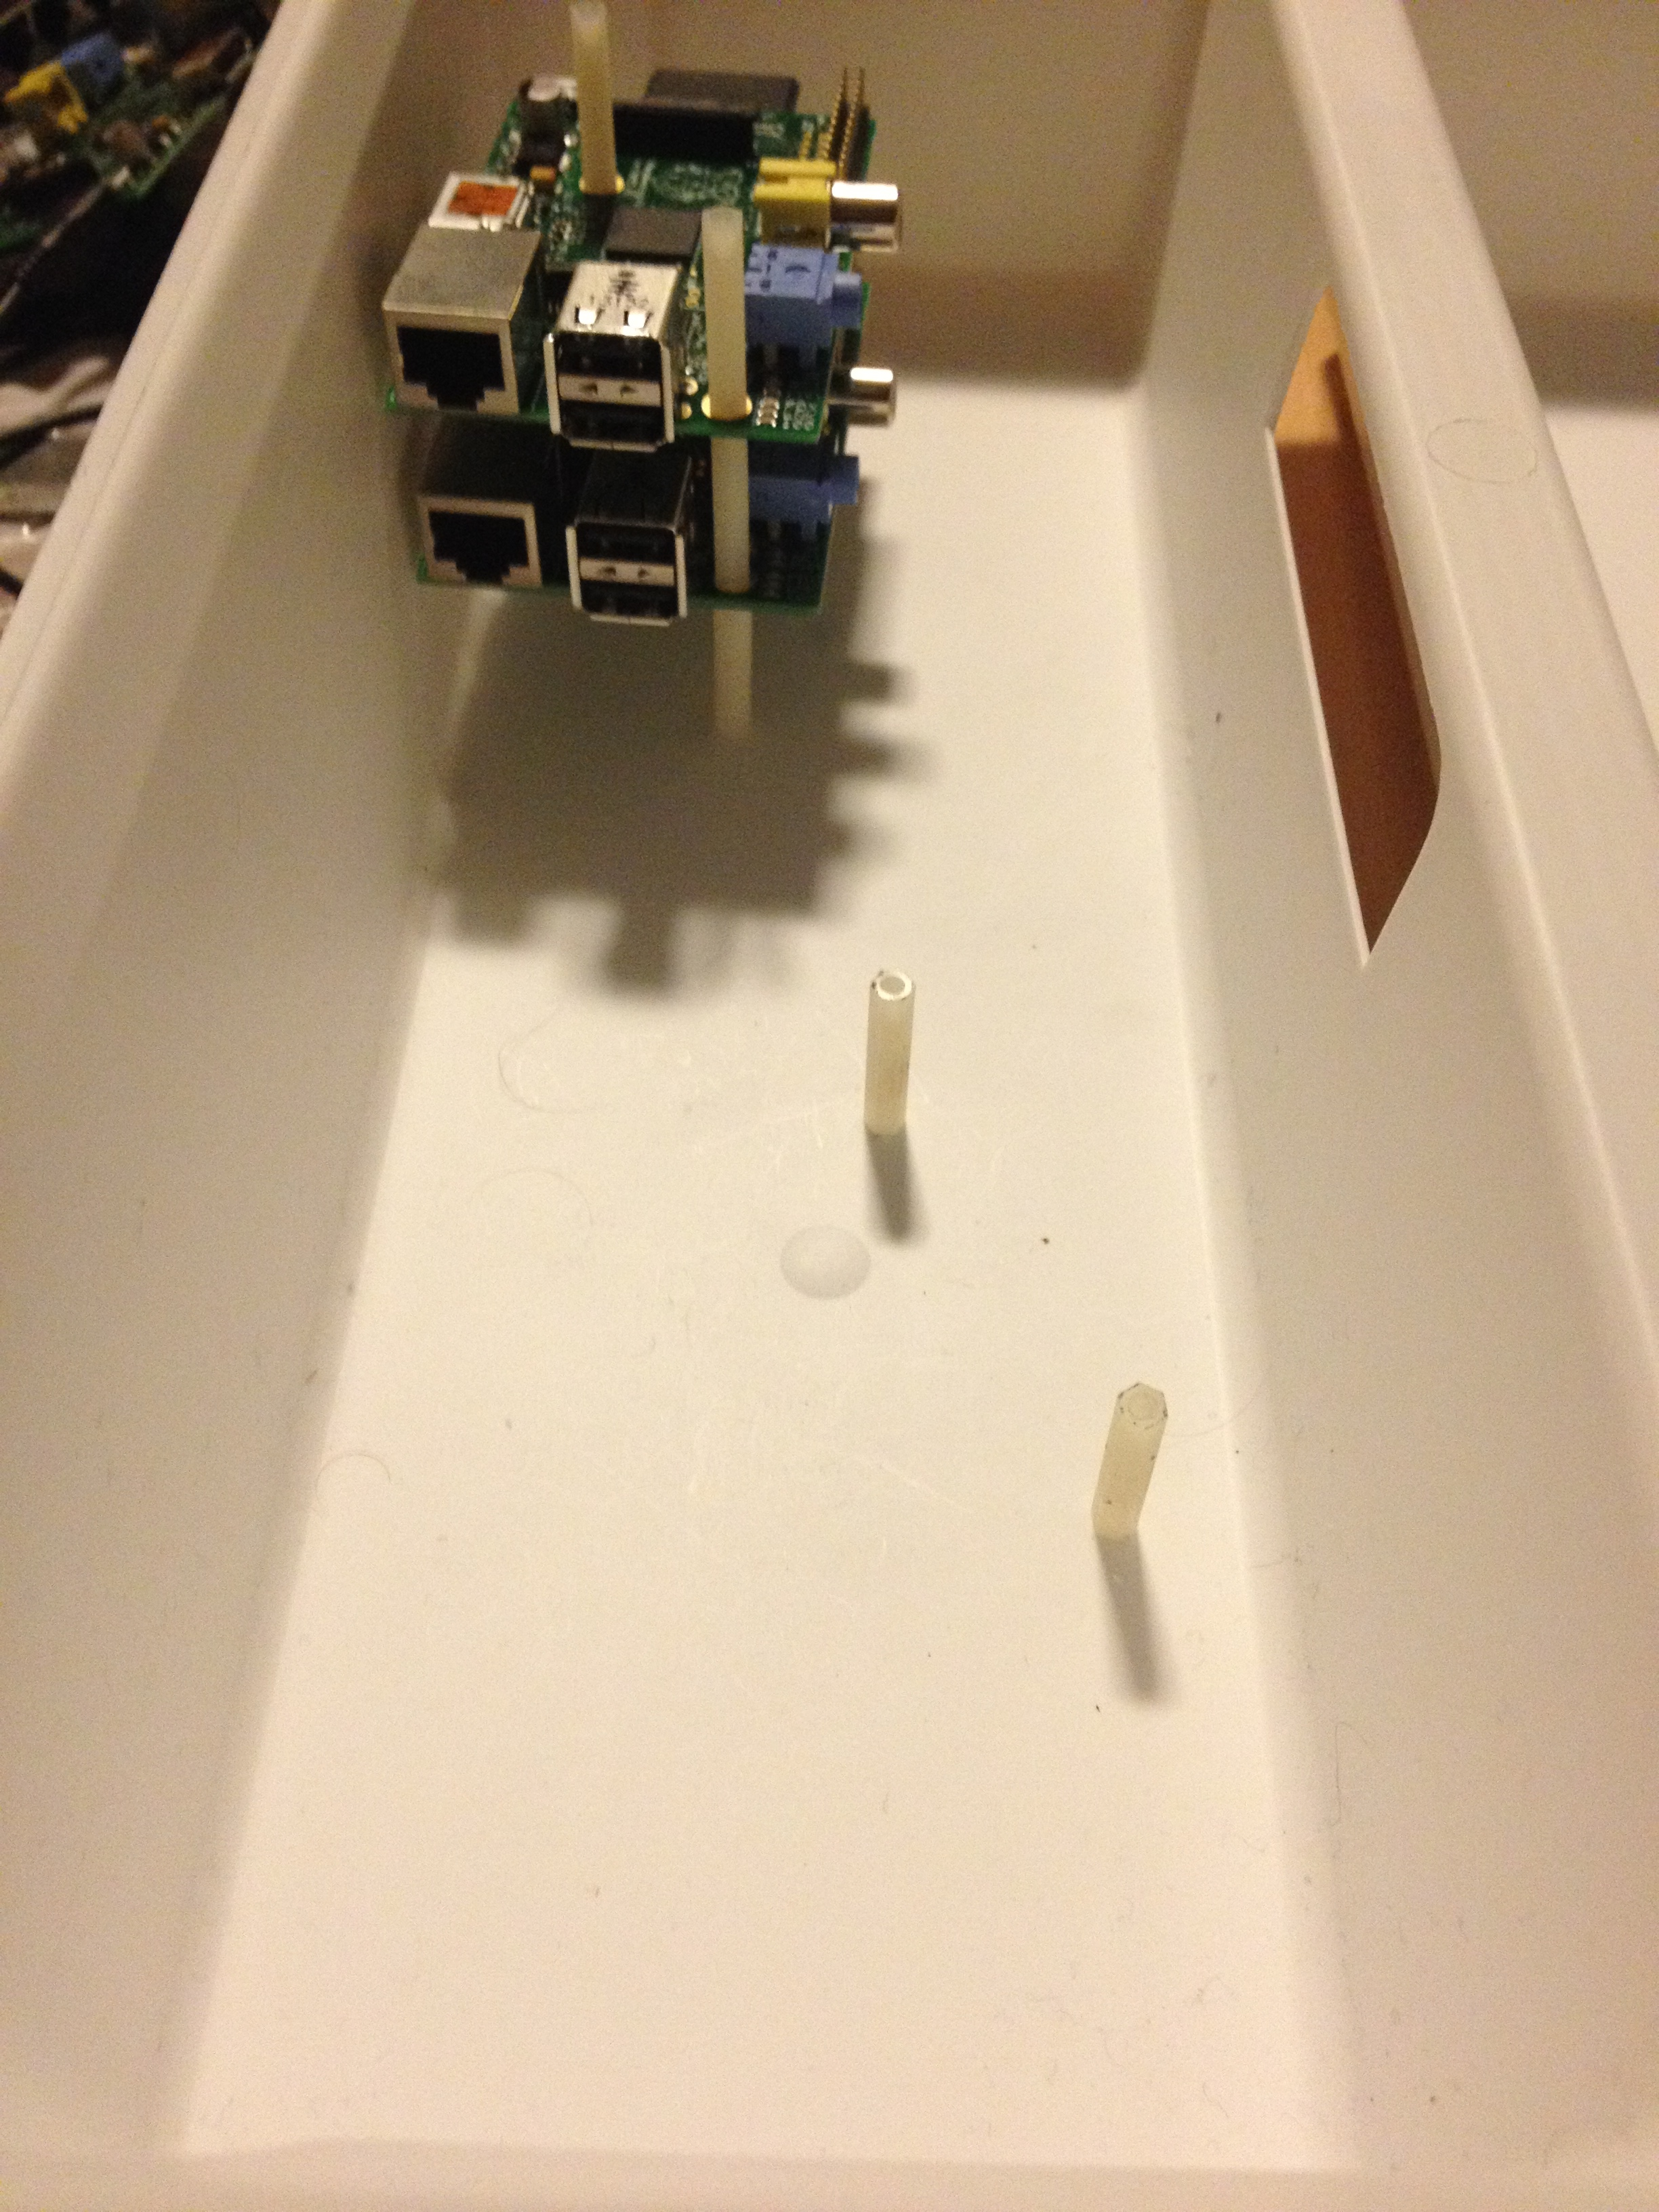
\includegraphics[width=0.5\textwidth]{thebuild/cluster_inside.jpg}
    \caption{Inside the clusterbox}
    \label{fig:build_cluster_inside}
\end{figure}




\clearpage

\section{Setup}
\label{sec:setup}

In this section we explain how we set up the experiments with the cluster to see how it performs. We will later list these results and discuss and compare these to results from a MacBook Pro Late 2012.

\subsection{Introduction}
We plan on running these experiments in two phases, first to identify areas where improvement can be made along with bottlenecks and then after attempting to mitigate these to see if any improvement was made, and see where we can end up.

We currently have 3 hardware configurations. The 8 node cluster can be split into:

\begin{enumerate}
\item 1 load distributor and 7 worker nodes
\item 8 worker nodes
\item 5 worker nodes (overclock)
\end{enumerate}

The overclock mode is reduced to 5 workers because the last 3 nodes refused to run properly at the overclocked speed, or didn't boot at all.

In addition we will also look at the i5 MacBook with 1 and 2 threads.

\subsection{Setup}
The setup is the cluster of 8 PI-nodes. Since we are limited by the 8 ports on our switch, we have the load distributor and the load generator connected to another D-Link router that is then connected to the switch.
Also note that we need to be wary of this bottlenecking our total bandwidth to the 7 worker nodes through one cable.
This means we can at most hope to push 100Mbit/s of data to the workers {\em in total}.
The network layout is illustrated in Figure \ref{fig:network}.

\begin{figure}[h]
    \centering
    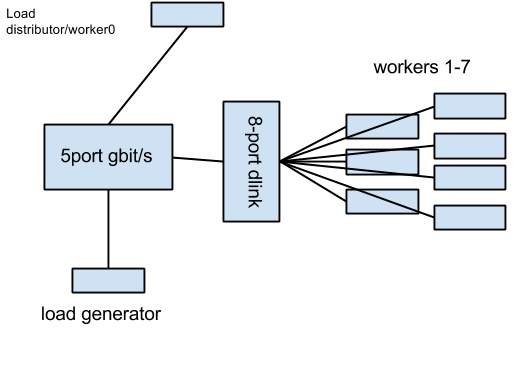
\includegraphics[width=0.8\textwidth]{experiments/networklayout}
    \caption{The network layout for the testing environment.}
    \label{fig:network}
\end{figure}


\subsection{Result gathering}
To obtain results we use a combination of controlling sending, output from the system and measuring the power consumed. To measure power usage we have a COITECH power consumption tool that is placed between the power outlet and our power adapters.
This lets us read the current power consumed by the whole system.

Our load generation utility has a few parameters for us to control. The number of queries to be sent, sending interval, number of threads and the set of nodes to which to send.

\subsection{MacBook Pro control}
When comparing on the MacBook, the load generator is run on a Mac Mini and the search program is run, either in one instance to test single core performance, or in two instances to utilize both the cores.
When running two instances these two operate on different ports.

\subsection{Overclocked Pis}
Overclocking is the process of making a computer operate at a faster clock rate than the manufacturer intended.
This is most often done by changing software parameters, typically by increasing the memory frequency, core frequency and/or operating voltage to make it stable at a higher clock rate.
Side effects of this process is an increase in power consumption and heat dissipation, and in some cases leads to system instability or even permanent damage to the components.

As it turns out every operation in our system is bounded by CPU speed, it would be reasonable to expect enhanced performance by overclocking the CPU.
The Raspberry PI is very simple to overclock. By editing boot config-file one can easily change the CPU parameters.

This file can be found under:

\begin{lstlisting}
\boot\config.txt
\end{lstlisting}

\begin{lstlisting}
## Some overclocking settings, cpu govenor is set to ondemand

##None
#arm_freq=700
#core_freq=250
#sdram_freq=400
#over_voltage=0

##Modest
#arm_freq=800
#core_freq=300
#sdram_freq=400
#over_voltage=0

##High
#arm_freq=950
#core_freq=450
#sdram_freq=450
#over_voltage=6

##Turbo
arm_freq=1000
core_freq=500
sdram_freq=600
over_voltage=6
\end{lstlisting}

We went for the Turbo mode, which is the fastest recommended mode by the creators of Raspberry Pi.
This mode doubles the memory frequency, and the GPU frequency which also drives the L2 cache for the CPU.
Doubling the L2 cache frequency is the main reason for this, with synthetic tests showing over 50\% gains in performance\cite{overclock}.
The L2 cache is really important as it is the main source of caching before the memory.

Unfortunately for us, only 5 of our units were able to run stably at the increased speed.
We saw both data corruption on the SD card, unable to completely boot.

\clearpage
\section{Results}
\label{sec:experiments}

Here follows our results from the testing.

\subsection{Maximum throughput}
We started out by looking at how many queries we could answer with the cluster, i.e. maximum throughput.

In order to find this we use a load generator which creates random queries and send these at various intervals to the cluster. As the traffic is UDP we expect to see a drop in answers from once the system is over saturated. The load generator is run on a lot more powerful computer outside the cluster.

We do this first by sending queries through a proxy of sorts, the load distributor, which chooses a random worker node to send the query to, then the worker sends the result back to the original client.
Later, we look at exposing direct worker access at the client.

\subsubsection{1 load distributor and 7 workers}
From the numbers in Table \ref{tab:cluster_load_dir} we see that there is a clear drop in performance at around 4400 requests per second. If we increase the load from this point we see a drastic loss in received responses. At this rate the load distributor is running on close to 100\% CPU while the workers are running at around 80\%. So we have reason to believe that the load distributor is holding back the system, effectively being the bottleneck.

\pgfplotstableread{../datasets/cluster_load_dir_requests.txt}\clusterloaddir
\begin{table}[h]
	\centering
	\pgfplotstabletypeset[
     	columns={requests, received},
     	every head row/.style={before row=\hline,
     	after row=\hline},
		every last row/.style={after row=\hline},
		columns/requests/.style={column name=Requests per second},
		columns/received/.style={column name=\% queries served},
     	]
    {\clusterloaddir}
	\caption{Maximum throughput with load distributor}
	\label{tab:cluster_load_dir}
\end{table}

\subsubsection{Required amount of nodes to deliver maximum throughput}
Since the load distributor appears to be a bottleneck in our system, it could be interesting to see how many workers we need to still be able to perform at maximum throughput, i.e. to see how many workers we can drop and still deliver the same amount of work.
In this experiment we have a look at the CPU utilization and query answer rate of the workers while gradually reducing the amount of workers in the cluster.

As suspected, when shutting down nodes one at a time and plotting performance at peak load, we first see an increase in dropped packets after 2 workers have been removed.

The full results are given in Table \ref{tab:clusterreduced}. We see that the cluster could run with 99.7\% of queries answered with 6 instead of 7 workers, and at 97.3\% answered queries with 5. With less than 5 workers, system performance degrades quickly with 78.2\% of queries answered at 4 workers.

We are quite happy with these results as they show that the work distribution looks fairly even. If we only needed a few nodes to handle the maximum throughput from the load distributor, there would be no use for 8 nodes in the cluster.

\pgfplotstableread{../datasets/cluster_reduced_workers_at_full_load.txt}\clusterreduced
\begin{table}
	\centering
	\pgfplotstabletypeset[
     	columns={workers, received},
     	every head row/.style={before row=\hline,
     	after row=\hline},
		every last row/.style={after row=\hline},
		columns/workers/.style={column name=Active working nodes},
		columns/received/.style={column name=\% queries served},
     	]
    {\clusterreduced}
	\caption{Performance when reducing working nodes}
\label{tab:clusterreduced}
\end{table}

\subsubsection{Power usage}
From similar work\cite{RPI_BEOWULF} we have seen that the Raspberry PI will drain up to 15\% more power under heavy load.

\pgfplotstableread{../datasets/watt_per_node.txt}\wattpernode
\begin{table}
	\centering
	\pgfplotstabletypeset[
     	columns={nodes, watt},
     	every head row/.style={before row=\hline,
     	after row=\hline},
		every last row/.style={after row=\hline},
		columns/nodes/.style={column name=Active Nodes},
		columns/watt/.style={column name=Watt},
     	]
    {\wattpernode}
	\caption{Watts consumed under load per node}
    \label{tab:wattpernode}
\end{table}

Despite having read that the Raspberry PIs would drain up to 15\% more energy under load, we were unable to have them drain more than about 9\% more. The cluster runs idle at 22-23W and 23-24W under load. These measurements include the switch which consumes a constant 4W. The power adapter that converts the power for the cluster also has a constant drain of 4W. This leads to the high initial drain we see for the first node.

One source of error for us is that the resolution on the measuring tool is not very high, it does not show decimals, and we do not know how rounding is handled.

\begin{figure}[!h]
\centering
	\begin{tikzpicture}
	\pgfplotstableread{../datasets/watt_per_node.txt}\wattpernode

	\begin{axis}
	[
	xlabel = active nodes,
	xmax = 9,
	xmin = 0,
	ylabel = consumption (W),
	ymax = 30,
	ymin = 0
	]
	\addplot table[y = watt] from \wattpernode ;
	\end{axis}
	\end{tikzpicture}
	\caption{Plot of power drain in the cluster. Shows linear scaling and the fairly high startup cost.}
\end{figure}

\subsubsection{Varying amount of nodes in the cluster}
We also want to vary the amount of nodes that are active in the cluster and plot performance and power consumption to see how it scales.
This is one of the more interesting experiments as one of the strengths of this cluster is that it is easy to power down nodes during hours of low load. We did not get to implement this feature, but it can be done. We will also plot the amount of queries we can deliver per watt used with differing numbers of nodes running.

As we can see from Table \ref{tab:cluster_reqwattnode} we have a steady increase in requests we can service per watt every time we add a node to the cluster. However, since adding any more nodes to the cluster would require a new power supply as well as more network equipment, further scaling would not be very effective, so this is our breakpoint.

\begin{figure}[!h]
\centering
	\begin{tikzpicture}
	\pgfplotstableread{../datasets/cluster_load_dist_request_watt_per_node.txt}\clusterreqwattnode

	\begin{axis}
	[
	xlabel = active nodes,
	xmax = 9,
	xmin = 0,
	ylabel = requests per Watt,
	ymax = 200,
	ymin = 0
	]
	\addplot table[y = reqwatt] from \clusterreqwattnode ;
	\end{axis}
	\end{tikzpicture}
	\caption{Plot showing the }
\end{figure}

\begin{table}
	\pgfplotstableread{../datasets/cluster_load_dist_request_watt_per_node.txt}
	\clusterreqwattnode
	\centering
	\pgfplotstabletypeset[
     	columns={nodes,request,	watt, reqwatt},
     	every head row/.style={before row=\hline,
     	after row=\hline},
		every last row/.style={after row=\hline},
		columns/requests/.style={column name=Requests per second},
		columns/watt/.style={column name=Watt},
		columns/reqwatt/.style={column name=Requests per watt},
     	]
    {\clusterreqwattnode}
	\caption{Efficieny with various nodes}
\label{tab:cluster_reqwattnode}
\end{table}

\subsubsection{Discussion}
After the first phase of testing we can draw some interesting conclusions. With regards to throughput there is a clear point where the system can't keep up with the traffic. At this point the load balancers UDP buffers are filling up and we lose queries.

We verified this by looking at the system network buffers while under load. In Linux, one can look at the buffer status with the command $$netstat -aupn$$, giving something like this:
\begin{lstlisting}[caption={Output of {\tt netstat -aupn | grep 32002}},captionpos=b,label={lst:netstat}]
Proto Recv   Send   Local Addres         Address     PID/name
udp   163840 163840 192.168.0.200:32002  0.0.0.0:*   296/bin/load_distri
\end{lstlisting}
In Listing \ref{lst:netstat} we see that the {\tt Recv} buffer and {\tt Send} buffer are currently containing 163840 bytes.
The maximum size of the buffer is given by {\tt /proc/sys/net/core/rmem\_max}. It is listed in bytes and can be modified with a {\tt sysctl} call: {\tt sysctl -w net.core.rmem\_max=value}.
As we can see in this example, the buffer is currently maxed out, and all additional packages will be lost. The load distributor can not handle any more load. Increasing the buffer size only lead to negligible improvements, as the buffer fills up very quickly.

We also see that the performance quickly diminishes as we increase the load. After the breakpoint, practically no additional queries get answered.
This is to be expected.

Our tests regarding energy consumption and scaling show that there is little difference in a Raspberry PI running idle and full load.
It's also of note that the network switch is at 4 watts responsible for 25\% of the consumed power in the cluster.
This would impact further scaling as it would remove the advantage of each PI improving the efficiency of the cluster.

\subsection{8 workers}
As we discovered in phase 1, the load balancer seems to be limiting the throughput of our cluster.
We therefore try to mitigate this by removing the load distributor entirely and rather have the load generating application (client) deal with distributing work.
This would also make it easier to compare with results of the same system running on the MacBook.

By moving the task of distributing load from the cluster and into the load generator (client library) we of course free up one node in the system, so we now have 8 working nodes for these tests. We expect this to improve our throughput and efficiency by a still linear amount, which we later confirm.

\subsubsection{Maximum throughput phase 2}
As we identified the load distributor as the bottleneck in our system we decided to move the load distribution out into the load generator.
This was implemented by having one thread in the client for each node in the cluster, sending queries at various intervals. The results from the load testing are given in Table \ref{tab:cluster_only_workers}.

\pgfplotstableread{../datasets/cluster_only_workers_requests.txt}\clusteronlyworkers
\begin{table}
	\centering
	\caption{Maximum throughput without load distributor}
	\pgfplotstabletypeset[
     	columns={requests, received},
     	every head row/.style={before row=\hline,
     	after row=\hline},
		every last row/.style={after row=\hline},
		columns/requests/.style={column name=Requests per second},
		columns/received/.style={column name=\% queries served},
     	]
    {\clusteronlyworkers}
\label{tab:cluster_only_workers}
\end{table}

\subsubsection{Scalability and energy efficiency}
As the system still consists of the same nodes doing work we don't expect there to be a change in power consumption, however since there now is 8 workers we should see an improvement in how efficient we can serve queries of various loads.
We will run the same test as in phase 1 where we try to find the breakpoint for the system at an increasing amount of nodes working.

\begin{table}
	\pgfplotstableread{../datasets/cluster_only_workers_request_watt_per_node.txt}
	\clusterworkerreqwatt
	\centering
	\pgfplotstabletypeset[
     	columns={nodes,requests, watt, reqwatt},
     	every head row/.style={before row=\hline,
     	after row=\hline},
		every last row/.style={after row=\hline},
		columns/nodes/.style={column name=Active nodes},
		columns/requests/.style={column name=Requests per second},
		columns/watt/.style={column name=Watt},
		columns/reqwatt/.style={column name=Requests per watt},
     	]
    {\clusterworkerreqwatt}
    \caption{Efficiency with various nodes without load balancer}
\label{tab:cluster_worker_req_watt}
\end{table}

As we can see in Table \ref{tab:cluster_worker_req_watt} we are able to achieve 181 requests per second per watt.
This is an increase of 20\%. This is of course mostly due to having an additional worker pulling its weight, but we are also able to push each individual node harder without the load balancer in place.

\subsubsection{Discussion}
When skipping the load distributor and using only worker nodes we see that it performs better, and a linear increase in performance is indeed observed.
We are now able to service up to around 5000 queries per second. This is an 13\% increase from the 7 workers plus 1 load distributer.
Along with the increase in maximum performance we also see that it behaves a lot better under higher loads.
If we compare the two methods we see that at around 6800 requests per second the load balancer is only able to serve around half its requests, while the cluster is answering 98\% of the requests without the load distributor.

\subsection{Mac VS Cluster of PIs}
In this section we will explore how our system performs compared to a MacBook Pro running the same software. We will again try to find the breakpoints of how much traffic the MacBook can handle and how efficient it can serve the requests. We test in two rounds. First only using 1 search process on the MacBook. This would then not utilize both cores on the CPU. Then we run two processes simultaneously and see how well that performs. We will also measure the power consumption on the mac under both idle and heavy load.

\subsubsection{Maximum throughput}
Running with one core we found the maximum throughput to at around 11000 requests per second. Over double the amount that of the cluster.
However this was to be expected with so much more powerful hardware. With two processes running we were able to push it up to 12700 requests per second. At this point we are pushing the limits of what both the network and the MacBook can handle.

\subsubsection{Energy}
Unlike the Raspberry PIs the MacBook really has a lot of power management built into it. We have measured it running idle at around 18 Watts and managed to push it up to 28 Watts while serving requests.
We also see that how many requests we send to it reflect in the amount of power it consumes. The results of this test can be found in Table \ref{tab:mac_energy_1core} and Table \ref{tab:mac_energy_2core}.

\begin{table}
	\pgfplotstableread{../datasets/mac_energy_1core.txt}
	\macenenrgyonecore
	\centering
	\pgfplotstabletypeset[
     	columns={requests, watt, reqwatt},
     	every head row/.style={before row=\hline,
     	after row=\hline},
		every last row/.style={after row=\hline},
		columns/requests/.style={column name=Requests per second},
		columns/watt/.style={column name=Watt},
		columns/reqwatt/.style={column name=Requests per watt},
     	]
    {\macenenrgyonecore}
    \caption{Mac efficiency 1 core}
\label{tab:mac_energy_1core}
\end{table}

\begin{table}
	\pgfplotstableread{../datasets/mac_energy_2core.txt}
	\macenergytwocore
	\centering
	\pgfplotstabletypeset[
     	columns={requests, watt, reqwatt},
     	every head row/.style={before row=\hline,
     	after row=\hline},
		every last row/.style={after row=\hline},
		columns/requests/.style={column name=Requests per second},
		columns/watt/.style={column name=Watt},
		columns/reqwatt/.style={column name=Requests per watt},
     	]
    {\macenergytwocore}
    \caption{Mac efficiency 2 core}
\label{tab:mac_energy_2core}
\end{table}

It is apparent that under maximum load not surprisingly there is no way the PI Cluster can contest the MacBook Pro other price.
However it is interesting to see how our system compares on lower request rates compared to the MacBook.
Request rates that are within the limits of our system, the system surprisingly performs comparable to the MacBook.

\subsubsection{Cold reads}
While all the other experiments have been performed on the cluster after a significant number of queries already has been answered. This ensured replicate-able results as we assume most the query words are already in memory and cache. However it would be interesting to see how the two compares when answering queries right after a reboot. In this experiment we send 5000 queries to each core operating, so in total 10000 for the MacBook and 40000 for the cluster. We then try pinpoint the breakpoint where the machines are unable to keep up with the load. The Pi cluster is run in the mode where all nodes are workers.

When measuring these numbers we ran into some interesting problems. For one, the sleep system call we use to limit the interval between queries is limited at milliseconds. This turned out to be a problem for measuring the performance of the MacBook Pro as its breakpoint lies somewhere between the minimum sleep duration and no sleep duration. This is reflected in table\ref{tab:coldread_mac} where we have a gap between a load we clearly can support and a load we clearly cannot support.

\begin{table}[h]
	\pgfplotstableread{../datasets/coldread_pi.txt}
	\coldreadpi
	\centering
	\pgfplotstabletypeset[
     	columns={nrps, nanswers, orps, oanswers},
     	every head row/.style={after row=\hline},
		every last row/.style={after row=\hline},
		columns/nrps/.style={column name=Rps},
		columns/nanswers/.style={column name=received(\%)},
		columns/orps/.style={column name=Rps(O)},
		columns/oanswers/.style={column name=received(\%)(O))},
     	]
    {\coldreadpi}
    \caption{Cold reads Pi cluster. Requests per second, and answers received in \%. (O) is with code optimization}
\label{tab:coldread_pi}
\end{table}

\begin{table}[h]
	\pgfplotstableread{../datasets/coldread_mac.txt}
	\coldreadmac
	\centering

	\pgfplotstabletypeset[
     	columns={nrps, nanswers, orps, oanswers},
     	every head row/.style={after row=\hline},
		every last row/.style={after row=\hline},
		columns/nrps/.style={column name=Rps},
		columns/nanswers/.style={column name=received(\%)},
		columns/orps/.style={column name=Rps(O)},
		columns/oanswers/.style={column name=received(\%)(O)},
     	]
    {\coldreadmac}
    \caption{Cold reads MacBook. Requests per second, and answers received in \%. (O) is with code optimization}
\label{tab:coldread_mac}
\end{table}

Without optimization the Pi cluster is able to support around 3000 requests per second. This is 60\% of the load it could handle previously. We also see that the code optimization does increase this number to 80\%.

The Macbook fared similarly. At only around 5500 rps the performance is halved. With the optimization the performance is somewhere between 7000 and 10000.

We did expect the cluster to gain some ground when we forced this much disk access. However as the MacBook runs on flash storage with reading speeds of up to 400MB/s and the poor Pis have SD-cards providing 5-8MB/s, the MacBook does have an unfair advantage.

\section{Overclocked Pis}
By changing from no over clocking to turbo mode we increase the clock frequency from 700MHz to 1000MHz. We also increase the GPU core frequency which drives the L2 cache.

As mentioned in the hardware section, overclocking the Raspberry PI might bring certain downsides. Users have experienced data corruption on the SD card as well as general instability. There are also reports of different degrees of tolerance among the Raspberry PIs. Some works perfectly under any degree of overclocking while others quickly start showing symptoms of instability.

We started out by overclocking one node and then run some tests. Everything seemed to work, so we added the overclocking parameters to the entire cluster. After then rebooting the cluster we experienced all the problems mentioned above. One node had problems with its SD-card and two others were struggling with booting or network access. We did however manage to find a stable set of five nodes to compare with our existing results. In this experiment we ran five individual workers similarly to when we tried to pin point the maximum performance of the cluster with various amounts of nodes.

We were able to see an increase in throughput of around 10\% with the cores overclocked. This number was a lot lower than expected taking into account that the cluster was using 21 watts compared to 16 without the overclock. At this rate the cluster can deliver 133 requests per watt, compared to 152 without the overclock. So this was generally bad value.


\section{Further optimization}
In an attempt to further improve our performance we have tried some optimization in our code. One of them being changing the load distributor from using $$rand() \bmod N,$$ where N is the number of nodes in the cluster, to just keeping iterating over the range 1-7 instead. We did however not notice any change from that.

Originally we always sent queries as 1024 byte messages. This was done for simplicity but of course at a cost of performance. By instead sending only as many bytes as needed we saw a dramatic increase in performance. Doing all measurements again was not an option but we did measure some values for comparison again.





















\section{Conclusions and further work}



\clearpage
\bibliographystyle{plain}
\bibliography{references}





\end{document}
